% !TeX spellcheck = hu_HU
% !TeX encoding = UTF-8
% !TeX program = xelatex
\documentclass[12pt,a4paper,oneside]{report}

% thanks to http://tex.stackexchange.com/a/47579/71109
\usepackage{ifxetex}
\usepackage{ifluatex}
\newif\ifxetexorluatex % a new conditional starts as false
\ifnum 0\ifxetex 1\fi\ifluatex 1\fi>0
  \xetexorluatextrue
\fi

\ifxetexorluatex
  \usepackage{fontspec}
\else
  \usepackage[T1]{fontenc}
  \usepackage[utf8]{inputenc}
  \usepackage[lighttt]{lmodern}
\fi

\usepackage[english,magyar]{babel} % Alapértelmezés szerint utoljára definiált nyelv lesz aktív, de később külön beállítjuk az aktív nyelvet.

%\usepackage{cmap}
\usepackage{amsfonts,amsmath,amssymb} % Mathematical symbols.
%\usepackage[ruled,boxed,resetcount,linesnumbered]{algorithm2e} % For pseudocodes. % beware: this is not compatible with LuaLaTeX, see http://tex.stackexchange.com/questions/34814/lualatex-and-algorithm2e
\usepackage{booktabs} % For publication quality tables for LaTeX
\usepackage{graphicx}

%\usepackage{fancyhdr}
%\usepackage{lastpage}

\usepackage{anysize}
%\usepackage{sectsty}
\usepackage{setspace} % For setting line spacing

\usepackage[unicode]{hyperref} % For hyperlinks in the generated document.
\usepackage{xcolor}
\usepackage{listings} % For source code snippets.

\usepackage[amsmath,thmmarks]{ntheorem} % Theorem-like environments.

\usepackage[hang]{caption}

\newcommand{\selecthungarian}{
  \selectlanguage{magyar}
  \setlength{\parindent}{2em}
  \setlength{\parskip}{0em}
  \frenchspacing
}

\newcommand{\selectenglish}{
  \selectlanguage{english}
  \setlength{\parindent}{0em}
  \setlength{\parskip}{0.5em}
  \nonfrenchspacing
  \renewcommand{\figureautorefname}{Figure}
  \renewcommand{\tableautorefname}{Table}
  \renewcommand{\partautorefname}{Part}
  \renewcommand{\chapterautorefname}{Chapter}
  \renewcommand{\sectionautorefname}{Section}
  \renewcommand{\subsectionautorefname}{Section}
  \renewcommand{\subsubsectionautorefname}{Section}
}

\usepackage[numbers]{natbib}
\usepackage{xspace}

\usepackage{xurl} % For breaking long URLs in the bibliography.

% js listing
\usepackage{listings}
\usepackage[many]{tcolorbox}
\usepackage{xcolor}

% colors
\definecolor{white}{rgb}{1,1,1}
\definecolor{black}{rgb}{0,0,0}
\definecolor{middlegray}{rgb}{0.5,0.5,0.5}
\definecolor{lightgray}{rgb}{.95,.95,.95}
\definecolor{arsenic}{rgb}{0.23, 0.27, 0.29}
\definecolor{arsenicLight}{rgb}{0.20, 0.20, 0.20}
\definecolor{darkgray}{rgb}{.4,.4,.4}
\definecolor{purple}{rgb}{0.65, 0.12, 0.82}
\definecolor{orange}{rgb}{0.8,0.3,0.3}
\definecolor{yac}{rgb}{0.6,0.6,0.1}
\definecolor{green}{rgb}{.2,0.6,0.3}
\definecolor{azure}{rgb}{0.0, 0.5, 1.0}
\definecolor{editorGray}{rgb}{0.95, 0.95, 0.95}
\definecolor{editorOcher}{rgb}{1, 0.5, 0}
\definecolor{editorGreen}{rgb}{0, 0.5, 0}
\definecolor{orange}{rgb}{1,0.45,0.13}
\definecolor{olive}{rgb}{0.17,0.59,0.20}
\definecolor{brown}{rgb}{0.69,0.31,0.31}
\definecolor{purple}{rgb}{0.38,0.18,0.81}
\definecolor{lightblue}{rgb}{0.1,0.57,0.7}
\definecolor{lightred}{rgb}{1,0.4,0.5}
\definecolor{amber}{rgb}{1.0, 0.75, 0.0}

\definecolor{vscodered}{HTML}{E53935}
\definecolor{vscodelightred}{HTML}{EF5350}
\definecolor{vscodeblue}{HTML}{1565C0}
\definecolor{vscodegreen}{HTML}{66BB6A}

\definecolor{lightblack}{HTML}{212121}
\definecolor{darkraspberry}{rgb}{0.53, 0.15, 0.34}

% blue hues
\definecolor{bleudefrance}{rgb}{0.19, 0.55, 0.91}
\definecolor{brandeisblue}{rgb}{0.0, 0.44, 1.0}
\definecolor{blue(ncs)}{rgb}{0.0, 0.53, 0.74}
\definecolor{coolblack}{rgb}{0.0, 0.18, 0.39}

% red hues
\definecolor{coralred}{rgb}{1.0, 0.25, 0.25}
\definecolor{darkred}{rgb}{0.55, 0.0, 0.0}

% general settings for listing
\lstset{
basicstyle=\normalsize\ttfamily,
basewidth  = {.5em,0.4em},
captionpos=t,
lineskip={2pt},
backgroundcolor=\color{white},
framextopmargin=6pt,
framexrightmargin=0.9em,
framexleftmargin=0.9em,
framexbottommargin=6pt,
frame=tb,
framerule=0pt,
framesep=6.5mm,
fillcolor=\color{white},
rulecolor=\color{middlegray},
numbers=left,
numberstyle=\normalfont\color{middlegray},
numbersep=16pt,
abovecaptionskip=-5pt, %space above the caption
belowcaptionskip=10pt, %space below the caption
extendedchars=true,
showstringspaces=false,
showspaces=false,
stepnumber=1, % the step between two line-numbers. If it is 1 each line will be numbered
tabsize=2,
breaklines=true,
showtabs=false,
upquote=true,
% German umlauts
literate=%
  {Ö}{{\"O}}1
{Ä}{{\"A}}1
{Ü}{{\"U}}1
{ß}{{\ss}}1
{ü}{{\"u}}1
{ä}{{\"a}}1
{ö}{{\"o}}1
}

% define language
\lstdefinelanguage{JavaScript}{
  keywords={typeof, new, true, false, catch, then, function, return, catch, switch, var, if, in, while, do, else, case, break, default, this, process},
  keywordstyle=\color{editorGreen}\bfseries,
  ndkeywords={class, export, boolean, throw, implements, import, from, const, async, await, private, public, readonly, static, constructor, get, set, yield, interface, type},
  ndkeywordstyle=\color{vscodeblue}\bfseries,
  identifierstyle=\color{black},
  sensitive=false,
  comment=[l]{//},
  morecomment=[s]{/*}{*/},
  commentstyle=\color{editorGreen}\ttfamily,
  stringstyle=\color{darkred}\ttfamily,
  morestring=[b]',
  morestring=[b]",
  morestring=*[d]`,
  moredelim=[s][]{\$\{}{\}},
  morekeywords=[3]{@UseGuards, @ApiFoundResponse, @ApiQuery, @Controller, @Injectable, @Module, @Inject, @Body, @Param, @Query, @UseInterceptors, @UseFilters, @UploadedFile, @UsePipes, @Get, @Post, @Put, @Delete, @Patch, @CurrentUser, @Res, @Next, @Headers, @Session, @Request, @All, string, number, null, void, undefined},
  keywordstyle={[3]\color{darkraspberry}\bfseries}
}

\lstdefinelanguage{SQL}{
  keywords={select, where, from},
  keywordstyle=\color{editorGreen}\bfseries,
  ndkeywords={},
  ndkeywordstyle=\color{vscodeblue}\bfseries,
  identifierstyle=\color{black},
  sensitive=false,
  comment=[l]{--},
  morecomment=[s]{/*}{*/},
  commentstyle=\color{editorGreen}\ttfamily,
  stringstyle=\color{darkred}\ttfamily,
  morestring=[b]',
  morestring=[b]"
}


\lstdefinelanguage{HTML5}{
  language=html,
  sensitive=true,
  alsoletter={<>=-},
  morecomment=[s]{<!-}{-->},
  tag=[s],
  otherkeywords={
      % General
      >,
      % Standard tags
      <!DOCTYPE,
      </html, <html, <head, <title, </title, <style, </style, <link, </head, <meta, />,
      % body
      </body, <body,
      % Divs
      </div, <div, </div>,
      % Paragraphs
      </p, <p, </p>,
      % scripts
      </script, <script,
      % More tags...
      <canvas, /canvas>, <svg, <rect, <animateTransform, </rect>, </svg>, <video, <source, <iframe, </iframe>, </video>, <image, </image>, <header, </header, <article, </article
    },
  ndkeywords={
      % General
      =,
      % HTML attributes
      charset=, src=, id=, width=, height=, style=, type=, rel=, href=,
      % SVG attributes
      fill=, attributeName=, begin=, dur=, from=, to=, poster=, controls=, x=, y=, repeatCount=, xlink:href=,
      % properties
      margin:, padding:, background-image:, border:, top:, left:, position:, width:, height:, margin-top:, margin-bottom:, font-size:, line-height:,
      % CSS3 properties
      transform:, -moz-transform:, -webkit-transform:,
      animation:, -webkit-animation:,
      transition:,  transition-duration:, transition-property:, transition-timing-function:,
    }
}

\lstdefinelanguage{Terraform}{
  keywords={terraform, variable, locals, output, module, resource, data, backend, true, false, var, local},
  keywordstyle=\color{vscodegreen}\bfseries,
  ndkeywords={lifecycle, provisioner, connection, length, lookup, merge, coalesce, zipmap, flatten, try, null, for, if, else, each, in, template_file, object, map, string, number, null_resource},
  ndkeywordstyle=\color{vscodeblue}\bfseries,
  sensitive=false,
  comment=[l]{\#},
  commentstyle=\color{editorGreen}\ttfamily,
  stringstyle=\color{darkred}\ttfamily,
  moredelim=[s][]{\$\{}{\}},
  morestring=[b]',
  morestring=*[d]",
  identifierstyle=\color{black}\ttfamily,
}

\lstdefinelanguage{Dockerfile}{
  keywords={FROM, RUN, COPY, ADD, ENTRYPOINT, CMD,  ENV, ARG, WORKDIR, EXPOSE, LABEL, USER, VOLUME, STOPSIGNAL, ONBUILD, MAINTAINER, HEALTHCHECK},
  keywordstyle=\color{vscodeblue}\bfseries,
  identifierstyle=\color{black},
  sensitive=false,
  comment=[l]{\#},
  commentstyle=\color{editorGreen}\ttfamily,
  stringstyle=\color{darkred}\ttfamily,
  morestring=[b]',
  morestring=[b]"
}

\lstdefinestyle{html} {%
% Code design
keywordstyle=\color{lightblack}\bfseries,
ndkeywordstyle=\color{lightblack}\bfseries,
identifierstyle=\color{lightblack},
commentstyle=\color{green}\ttfamily,
stringstyle=\color{darkred}\ttfamily,
% Code
language=HTML5,
%  alsolanguage=JavaScript,
alsodigit={.:;},
tabsize=2,
showtabs=false,
showspaces=false,
showstringspaces=false,
extendedchars=true,
breaklines=true,
% German umlauts
literate=%
  {Ö}{{\"O}}1
{Ä}{{\"A}}1
{Ü}{{\"U}}1
{ß}{{\ss}}1
{ü}{{\"u}}1
{ä}{{\"a}}1
{ö}{{\"o}}1
}

\lstdefinelanguage{CSS}
{morekeywords={color,background,margin,padding,margin,padding,font,weight,display,position,top,left,right,bottom,list,style,border,size,white,space,min,width, 	transition},
  sensitive=false,
  morecomment=[l]{//},
  morecomment=[s]{/*}{*/},
  morestring=[b]",
}

\newcommand\YAMLcolonstyle{\color{darkred}\mdseries}
\newcommand\YAMLkeystyle{\color{black}\bfseries}
\newcommand\YAMLvaluestyle{\color{vscodeblue}\mdseries}

\lstdefinelanguage{YAML}{
  keywords={true,false,null,y,n},
  keywordstyle=\color{darkgray}\bfseries,
  basicstyle=\YAMLkeystyle,                                 % assuming a key comes first
  sensitive=false,
  comment=[l]{\#},
  morecomment=[s]{/*}{*/},
  commentstyle=\color{editorGreen}\ttfamily,
  stringstyle=\YAMLvaluestyle\ttfamily,
  % moredelim=[l][\color{orange}]{\&},
  moredelim=[l][\color{magenta}]{*},
  moredelim=**[il][\YAMLcolonstyle{:}\YAMLvaluestyle]{:},   % switch to value style at :
  morestring=[b]',
  morestring=[b]",
  literate =    {---}{{\ProcessThreeDashes}}3
  {>}{{\textcolor{red}\textgreater}}1
  {|}{{\textcolor{red}\textbar}}1
  {\ -\ }{{\mdseries\ -\ }}3,
}

\lstdefinestyle{css} {
  language=CSS,
  keywordstyle=\color{lightblack},
}

\lstdefinestyle{js} {
  language=JavaScript
}

\lstdefinestyle{tf} {
  language=Terraform
}

\lstdefinestyle{dockerfile} {
  language=Dockerfile
}

\lstdefinestyle{yaml} {
  language=YAML
}

\lstdefinestyle{sql} {
  language=SQL,
  keywordstyle=\color{azure}
}

% Hyphenation rules
\hyphenation{PostgreSQL Cloud-Front strea-ming stream pa-cket Apple Lambda Edge Route Node Vite Actions Action Type-Script Java-Script-ből Java-Script React Function Rou-ter route table build buil-del Re-quest bucket re-po-si-to-ry Docker Registry Se-cu-ri-ty Group Gate-way Cloud-Watch AuthSCH OAuth Chrome Google Media-Package Media-Live back-end front-end}


\onehalfspacing % Set line spacing to 1.5

\newcommand{\vikszerzoVezeteknev}{Piller}
\newcommand{\vikszerzoKeresztnev}{Trisztán}

\newcommand{\vikkonzulensAMegszolitas}{}
\newcommand{\vikkonzulensAVezeteknev}{Kövesdán}
\newcommand{\vikkonzulensAKeresztnev}{Gábor}

\newcommand{\vikkonzulensBMegszolitas}{}
\newcommand{\vikkonzulensBVezeteknev}{}
\newcommand{\vikkonzulensBKeresztnev}{}

\newcommand{\vikkonzulensCMegszolitas}{}
\newcommand{\vikkonzulensCVezeteknev}{}
\newcommand{\vikkonzulensCKeresztnev}{}

\newcommand{\vikcim}{Videó streaming szolgáltatások implementációja}
\newcommand{\viktanszek}{\bmeaut} 
\newcommand{\vikdoktipus}{\msc}
\newcommand{\vikmunkatipusat}{diplomatervet} 

%--------------------------------------------------------------------------------------
% TDK-specifikus változók
%--------------------------------------------------------------------------------------
\newcommand{\tdkszerzoB}{Második Szerző} % Második szerző neve; hagyd üresen, ha egyedül írtad a TDK-t.
\newcommand{\tdkev}{2014} % A dolgozat írásának éve (pl. "2014") (Ez OTDK-nál eltérhet az aktuális évtől.)

% További adatok az OTDK címlaphoz (BME-s TDK-hoz nem kell kitölteni)
\newcommand{\tdkevfolyamA}{IV} % Első szerző évfolyama, római számmal (pl. IV).
\newcommand{\tdkevfolyamB}{III} % Második szerző évfolyama, római számmal (pl. III).
\newcommand{\tdkkonzulensbeosztasA}{egyetemi tanár} % Első konzulens beosztása (pl. egyetemi docens)
\newcommand{\tdkkonzulensbeosztasB}{doktorandusz} % Második konzulens beosztása (pl. egyetemi docens)

\newcommand{\szerzoMeta}{\vikszerzoVezeteknev{} \vikszerzoKeresztnev} 

%--------------------------------------------------------------------------------------
% Elnevezések
%--------------------------------------------------------------------------------------
\newcommand{\bme}{Budapesti Műszaki és Gazdaságtudományi Egyetem}
\newcommand{\vik}{Villamosmérnöki és Informatikai Kar}

\newcommand{\bmemit}{Méréstechnika és Információs Rendszerek Tanszék}
\newcommand{\bmeaut}{Automatizálási és Alkalmazott Informatikai Tanszék}

\newcommand{\keszitette}{Készítette}
\newcommand{\konzulens}{Konzulens}

\newcommand{\bsc}{Szakdolgozat}
\newcommand{\msc}{Diplomaterv}
\newcommand{\tdk}{TDK dolgozat}
\newcommand{\bsconlab}{BSc Önálló laboratórium}
\newcommand{\msconlabi}{MSc Önálló laboratórium 1.}
\newcommand{\msconlabii}{MSc Önálló laboratórium 2.}

\newcommand{\pelda}{Példa}
\newcommand{\definicio}{Definíció}
\newcommand{\tetel}{Tétel}

\newcommand{\bevezetes}{Bevezetés}
\newcommand{\koszonetnyilvanitas}{Köszönetnyilvánítás}
\newcommand{\fuggelek}{Függelék}

% Opcionálisan átnevezhető címek
%\addto\captionsmagyar{%
%\renewcommand{\listfigurename}{Saját ábrajegyzék cím}
%\renewcommand{\listtablename}{Saját táblázatjegyzék cím}
%\renewcommand{\bibname}{Saját irodalomjegyzék név}
%}

\newcommand{\szerzo}{\vikszerzoVezeteknev{} \vikszerzoKeresztnev}
\newcommand{\vikkonzulensA}{\vikkonzulensAMegszolitas\vikkonzulensAVezeteknev{} \vikkonzulensAKeresztnev}
\newcommand{\vikkonzulensB}{\vikkonzulensBMegszolitas\vikkonzulensBVezeteknev{} \vikkonzulensBKeresztnev}
\newcommand{\vikkonzulensC}{\vikkonzulensCMegszolitas\vikkonzulensCVezeteknev{} \vikkonzulensCKeresztnev}

\newcommand{\selectthesislanguage}{\selecthungarian}

\bibliographystyle{huplain}

\def\lstlistingname{lista}

\newcommand{\appendixnumber}{6}  % a fofejezet-szamlalo az angol ABC 6. betuje (F) lesz

%--------------------------------------------------------------------------------------
% Page layout setup
%--------------------------------------------------------------------------------------
% we need to redefine the pagestyle plain
% another possibility is to use the body of this command without \fancypagestyle
% and use \pagestyle{fancy} but in that case the special pages
% (like the ToC, the References, and the Chapter pages)remain in plane style

\pagestyle{plain}
\marginsize{35mm}{25mm}{15mm}{15mm}

\setcounter{tocdepth}{3}
%\sectionfont{\large\upshape\bfseries}
\setcounter{secnumdepth}{3}

\sloppy % Margón túllógó sorok tiltása.
\widowpenalty=10000 \clubpenalty=10000 %A fattyú- és árvasorok elkerülése
\def\hyph{-\penalty0\hskip0pt\relax} % Kötőjeles szavak elválasztásának engedélyezése


%--------------------------------------------------------------------------------------
% Setup hyperref package
%--------------------------------------------------------------------------------------
\hypersetup{
    % bookmarks=true,            % show bookmarks bar?
    unicode=true,              % non-Latin characters in Acrobat's bookmarks
    pdftitle={\vikcim},        % title
    pdfauthor={\szerzoMeta},    % author
    pdfsubject={\vikdoktipus}, % subject of the document
    pdfcreator={\szerzoMeta},   % creator of the document
    pdfproducer={},    % producer of the document
    pdfkeywords={},    % list of keywords (separate then by comma)
    pdfnewwindow=true,         % links in new window
    colorlinks=true,           % false: boxed links; true: colored links
    linkcolor=black,           % color of internal links
    citecolor=black,           % color of links to bibliography
    filecolor=black,           % color of file links
    urlcolor=black             % color of external links
}


%--------------------------------------------------------------------------------------
% Set up listings
%--------------------------------------------------------------------------------------
\definecolor{lightgray}{rgb}{0.95,0.95,0.95}
\lstset{
	basicstyle=\scriptsize\ttfamily, % print whole listing small
	keywordstyle=\color{black}\bfseries, % bold black keywords
	identifierstyle=, % nothing happens
	% default behavior: comments in italic, to change use
	% commentstyle=\color{green}, % for e.g. green comments
	stringstyle=\scriptsize,
	showstringspaces=false, % no special string spaces
	aboveskip=3pt,
	belowskip=3pt,
	backgroundcolor=\color{lightgray},
	columns=flexible,
	keepspaces=true,
	escapeinside={(*@}{@*)},
	captionpos=b,
	breaklines=true,
	frame=single,
	float=!ht,
	tabsize=2,
	literate=*
		{á}{{\'a}}1	{é}{{\'e}}1	{í}{{\'i}}1	{ó}{{\'o}}1	{ö}{{\"o}}1	{ő}{{\H{o}}}1	{ú}{{\'u}}1	{ü}{{\"u}}1	{ű}{{\H{u}}}1
		{Á}{{\'A}}1	{É}{{\'E}}1	{Í}{{\'I}}1	{Ó}{{\'O}}1	{Ö}{{\"O}}1	{Ő}{{\H{O}}}1	{Ú}{{\'U}}1	{Ü}{{\"U}}1	{Ű}{{\H{U}}}1
}


%--------------------------------------------------------------------------------------
% Set up theorem-like environments
%--------------------------------------------------------------------------------------
% Using ntheorem package -- see http://www.math.washington.edu/tex-archive/macros/latex/contrib/ntheorem/ntheorem.pdf

\theoremstyle{plain}
\theoremseparator{.}
\newtheorem{example}{\pelda}

\theoremseparator{.}
%\theoremprework{\bigskip\hrule\medskip}
%\theorempostwork{\hrule\bigskip}
\theorembodyfont{\upshape}
\theoremsymbol{{\large \ensuremath{\centerdot}}}
\newtheorem{definition}{\definicio}

\theoremseparator{.}
%\theoremprework{\bigskip\hrule\medskip}
%\theorempostwork{\hrule\bigskip}
\newtheorem{theorem}{\tetel}


%--------------------------------------------------------------------------------------
% Some new commands and declarations
%--------------------------------------------------------------------------------------
\newcommand{\code}[1]{{\upshape\ttfamily\scriptsize\indent #1}}
\newcommand{\doi}[1]{DOI: \href{http://dx.doi.org/\detokenize{#1}}{\raggedright{\texttt{\detokenize{#1}}}}} % A hivatkozások közt így könnyebb DOI-t megadni.

\DeclareMathOperator*{\argmax}{arg\,max}
%\DeclareMathOperator*[1]{\floor}{arg\,max}
\DeclareMathOperator{\sign}{sgn}
\DeclareMathOperator{\rot}{rot}


%--------------------------------------------------------------------------------------
% Setup captions
%--------------------------------------------------------------------------------------
\captionsetup[figure]{
	width=.75\textwidth,
	aboveskip=10pt}

\renewcommand{\captionlabelfont}{\bf}
%\renewcommand{\captionfont}{\footnotesize\it}

%--------------------------------------------------------------------------------------
% Hyphenation exceptions
%--------------------------------------------------------------------------------------
\hyphenation{Shakes-peare Mar-seilles ár-víz-tű-rő tü-kör-fú-ró-gép}


\author{\vikszerzo}
\title{\viktitle}

\begin{document}

\pagenumbering{gobble}

% %--------------------------------------------------------------------------------------
% Feladatkiiras (a tanszeken atveheto, kinyomtatott valtozat)
%--------------------------------------------------------------------------------------
\clearpage
\begin{center}
\large
\textbf{FELADATKIÍRÁS}\\
\end{center}

A feladatkiírást a tanszéki adminisztrációban lehet átvenni, és a leadott munkába eredeti, tanszéki pecséttel ellátott és a tanszékvezető által aláírt lapot kell belefűzni (ezen oldal \emph{helyett}, ez az oldal csak útmutatás). Az elektronikusan feltöltött dolgozatban már nem kell beleszerkeszteni ezt a feladatkiírást.


\selectthesislanguage
\hypersetup{pageanchor=false}
%--------------------------------------------------------------------------------------
%	The title page
%--------------------------------------------------------------------------------------
\begin{titlepage}
\begin{center}

\includegraphics[width=60mm,keepaspectratio]{figures/bme_logo.pdf}\\
\vspace{0.3cm}
\textbf{\bme}\\
\textmd{\vik}\\
\textmd{\viktanszek}\\[5cm]

\vspace{0.4cm}
{\huge \bfseries \vikcim}\\[0.8cm]
\vspace{0.5cm}
\textsc{\Large \vikdoktipus}\\[4cm]

{
	\renewcommand{\arraystretch}{0.85}
	\begin{tabular}{cc}
	 \makebox[7cm]{\emph{\keszitette}} & \makebox[7cm]{\emph{\konzulens}} \\ \noalign{\smallskip}
	 \makebox[7cm]{\szerzo} & \makebox[7cm]{\vikkonzulensA} \\
	  & \makebox[7cm]{\vikkonzulensB} \\
	  & \makebox[7cm]{\vikkonzulensC} \\
	\end{tabular}
}

\vfill
{\large \today}
\end{center}
\end{titlepage}
\hypersetup{pageanchor=false}

	
\tableofcontents\vfill

\selectlanguage{magyar}
\pagenumbering{gobble}
%--------------------------------------------------------------------------------------
% Nyilatkozat
%--------------------------------------------------------------------------------------
\begin{center}
\large
\textbf{HALLGATÓI NYILATKOZAT}\\
\end{center}

Alulírott \emph{\vikszerzoVezeteknev{} \vikszerzoKeresztnev}, szigorló hallgató kijelentem, hogy ezt a \vikmunkatipusat{} meg nem engedett segítség nélkül, saját magam készítettem, csak a megadott forrásokat (szakirodalom, eszközök stb.) használtam fel. Minden olyan részt, melyet szó szerint, vagy azonos értelemben, de átfogalmazva más forrásból átvettem, egyértelműen, a forrás megadásával megjelöltem.

Hozzájárulok, hogy a jelen munkám alapadatait (szerző(k), cím, angol és magyar nyelvű tartalmi kivonat, készítés éve, konzulens(ek) neve) a BME VIK nyilvánosan hozzáférhető elektronikus formában, a munka teljes szövegét pedig az egyetem belső hálózatán keresztül (vagy autentikált felhasználók számára) közzétegye. Kijelentem, hogy a benyújtott munka és annak elektronikus verziója megegyezik. Dékáni engedéllyel titkosított diplomatervek esetén a dolgozat szövege csak 3 év eltelte után válik hozzáférhetővé.

\begin{flushleft}
\vspace*{1cm}
Budapest, \today
\end{flushleft}

\begin{flushright}
 \vspace*{1cm}
 \makebox[7cm]{\rule{6cm}{.4pt}}\\
 \makebox[7cm]{\emph{\vikszerzoVezeteknev{} \vikszerzoKeresztnev}}\\
 \makebox[7cm]{hallgató}
\end{flushright}
\thispagestyle{empty}

\vfill
\clearpage
\thispagestyle{empty} % an empty page

\selectthesislanguage

\pagenumbering{roman}
\setcounter{page}{1}

\selecthungarian

%----------------------------------------------------------------------------
% Abstract in Hungarian
%----------------------------------------------------------------------------
\chapter*{Kivonat}\addcontentsline{toc}{chapter}{Kivonat}

Az IT szakma meghatározó kihívása a magasan teljesítőképes, könnyen skálázódó és stabil infrastruktúra létesítése különféle üzleti célok megvalósítására. A hírközlés, a média és a szórakoztatatás iparágaiban is kiemelt figyelmet kap ez a kihívás.

Ezek a virágzó és feltörekvő iparágak folyamatosan igénylik az olyan szoftverfejlesztőket, akik ezekre az iparágakra specializáltan is folyamatosan képzik magukat, valamint mélyen ismerik a szakterület technológiáit.

Diplomatervem célja demonstrálni egy az Amazon Web Services platformján futó felhő alapú médiaszolgáltatás-rendszer alapos tervezésének, implementálásának, valamint tesztelésének folyamatát. A rendszer a videó streaming szolgáltatások területén nyújt weben elérhető megoldást, és a felhasználók számára lehetővé teszi, hogy saját időbeosztásuknak megfelelően férjenek hozzá videótartalmakhoz (Video-on-Demand), valami élő adásokat is tudjanak megtekinteni (live streaming).

A megoldás ismertetése során kiemelt fókuszt kap a komponensek közötti laza kapcsolás kialakítása, az IT biztonsági kockázatok kezelése, az konfigurációmenedzsment fenntarthatósága. Felhasználásra kerülnek modern webes technológiák és DevOps technikák, mint a konténerizáció, a serverless függvények, a CI/CD csővezetékek és az Infrastructure as Code.

\vfill
\selectenglish

%----------------------------------------------------------------------------
% Abstract in English
%----------------------------------------------------------------------------
\chapter*{Abstract}\addcontentsline{toc}{chapter}{Abstract}

A key challenge for the IT profession is to build highly performant, easily scalable and stable infrastructure to support a variety of business goals. This challenge is also a major focus in Telecommunications, also in the Media \& Entertainment industry.

These booming and emerging industries are in constant need of software developers who train themselves continuously for these industries and have a deep knowledge of the technologies in the field.

My thesis project aims to demonstrate the process of thoroughly designing, implementing and testing a cloud-based media delivery system running on the Amazon Web Services platform. The system will provide a web-based solution for video streaming services, allowing users to access Video-on-Demand content and live streams.

The solution will focus on the design of loose coupling between components, the management of IT security risks and the sustainability of configuration management. Modern web technologies and DevOps techniques such as containerisation, serverless functions, CI/CD pipelines and Infrastructure as Code will be used.

\vfill
\selectthesislanguage

\newcounter{romanPage}
\setcounter{romanPage}{\value{page}}
\stepcounter{romanPage}


\pagenumbering{arabic}

%TODO import your own content
\chapter{\bevezetes}

\section{A témaválasztás indoklása}

Arról írok, hogy miért választottam a témát: Érdemesnek tartom a szakterület vizsgálatát, a média streaming maga elég szűk területe a szoftveres világnak, mégis roppant nagy szaktudást lehet benne felvenni. Médiaszolgáltatások fejlesztésének infrastrukturális és szoftveres igényei jelentős kihívást jelentenek a szakma architektjei számára, és a témában való elmélyülés nagyban hozzájárulhat a szakmai tudásom bővítéséhez.

\section{Kihívások a tématerületen}

Ez a szekció arról fog szólni, hogy szoftver architekteknek milyen kihívásokkal kell szembenézniük, ha egy olyan kaliberű szórakoztató médiaszolgáltatás-rendszert kell megtervezniük, mint a Netflix vagy a Twitch. 

Fel lesz sorolva jó pár dolog (felhasználói élmény szintre emelése, gyorsan fejlődő protokollok, különféle hardverekre/platformokra való optimalizálás, globális forgalmazás), kiemelve hogy én a biztonságra, a skálázhatóságra, az alaposan megtervezett és fenntartott infrastruktúrára helyezem a hangsúlyt. 


\chapter{Technológiai áttekintés}

\section{A videó streaming protokolljai}

Itt jó sok alszekcióban kifejtem a legfontosabb end-to-end protokollcsaládjait a streamingnek. Szó lesz az RTP/RTMP (és annak pull és push változatáról), a HLS/DASH, a WebRTC protokollokról. Ezek kardinalitása (források és felhasználók számát is figyelembe véve!) és a különféle alkalmazási területeik lesznek a fókuszban. Felmerül, hol működik az ABR (Adaptive Bitrate Streaming).

\section{Amazon Web Services}

Bevezető az AWS szolgáltatások világába, röviden bemutatom, hogy épül fel egy AWS account, milyen szolgáltatáscsoportokat ajánl, mivel lehet korlátozni a hozzáférést, az erőforrások akár egymás közötti kommunikációjá irányítani.

\subsection{Hagyományos webalkalmazások erőforrásai AWS-en}

Cloudfront mint CDN, S3 mint objektumtároló, RDS mint relációs adatbázis, Lambda mint szerver nélküli függvény, VPC mint privát hálózat, IAM mint hozzáféréskezelés, WAF mint web application firewall, Route53 mint DNS szolgáltatás.

\subsection{Videó streaming AWS-en}

Ebben pedig a már konkrét felhasznált (és nem felhasznált) AWS szolgáltatásokat mutatom be, mint a MediaLive, MediaPackage, és melyiket miért választottam, és a többit (IVS, saját konténerizált ffmpeg szerver) miért nem.

\section{A webes komponensek technológiái}

Ebben a részben a konkrét AWS-beli PaaS és FaaS szolgáltatásokon futó több rétegű appok választott technológiáit mutatom be: Node.js, React, Prisma, Postgres.

\subsection{TypeScript és JavaScript nyelvek}

Miért választottam a TypeScriptet, miért jobb a JavaScriptnél, felhasználása a JavaScriptnek a Lambda és Cloudfront Function-ökben.

\subsection{Node.js ökoszisztéma}

Node.js futtatókörnyezet, NestJS keretrendszer, Prisma ORM, AWS SDK.

\subsection{React és társkönyvtárai}

React, React Hook Forms, React Query, Vite.js, TailwindCSS.

\subsection{PostgreSQL}

Hasznos, mert open source, sok helyen elérhető DBMS motor.

\chapter{A tervezett felhőarchitektúra}

Gyors bevezető arról, hogy külön AWS accountba dolgoztam és felügyeltem a költségeim.

\section{Követelmények}

Funkcionális és nem-funkcionális követelmények, a rendszerrel szemben támasztott elvárások. Event driven architektúra (kiterjeszthetőség érdekében), skálázhatóság, biztonság, megbízhatóság.

\section{Logikai felépítés}

High-level leírása az AWS accounton belüli/datacenteren belüli hálózati kommunikáció rétegeinek.

\section{Video-on-Demand kiszolgálás folyamata}

High-level leírása a VoD kiszolgálás folyamatának, megemlítve, melyik választott szolgáltatások vesznek részt ebben.

\section{Live streaming folyamata}

High-level leírása a live streaming folyamatának, megemlítve, melyik választott szolgáltatások vesznek részt ebben.

\section{Konfigurációmenedzsment}

Terraform választásának indoklása. Kialakított Terragrunt module rendszer. GitHub actions a Terraform tervek előnézetére, OIDC felállítása az AWS role felvételére.

\chapter{Kliens közeli komponensek implementációja}

\section{A CDN és a hozzácsatolt erőforrások}

A CDN és az originjeinek tárgyalása, melyik origin mire való. VPC Origin tárgyalása, annak haszna. A WAF szerepe, a felkapcsolt cert és WAF web ACL szerepe.

\section{A statikus weboldal}

Az S3 bucketee. A statikus website kiszolgálásának módja.

\subsection{A React alkalmazás fejlesztése}

Fejlesztés részletei. Nem annyira lényeges most ebben a dolgozatban, de néhány szép kihívást jelentő kidolgozott form és egyebeket be lehet itt mutatni.

\subsection{A weboldal telepítésének CI/CD folyamata}

GitHub Actions a smoke tesztekre, workflowk, a deploymentek. Értsd itt: S3 telepítés.

\section{Média erőforrások objektumtárolói}

Hogy lettek felkonfigurálva és miért az egyes S3 bucket-ok (bucket policy, CORS policy).

\section{Elemental MediaLive és MediaPackage a live streamingben}

Az Elemental stack részeinek felkonfigurálása, a MediaLive channel és a MediaPackage channel felépítése, a MediaPackage endpoint konfigurálása. Miként kerül kiszolgálásra, melyiket mire használom. OBS bekötésének módja.

\chapter{Szerver oldali folyamatok implementációi}

\section{A virtuális privát felhő komponensei}

A VPC-beli (Virtual Private Cloud) subnetek, a security groupok, route táblák. A biztonság vizsgálata.

\section{A Node.js alkalmazás fejlesztése}

Fejlesztés részletei. Kitérve arra, hogy miképp könnyíti a munkát a Prisma, milyen egyéb szolgáltatások kerültek be, mi a felépítése a reponak, miért választottam ezt a stacket. S3 bucketba való mentése a videónak egy érdekes rész. Itt lehet szó az adatbázisbeli entitásokról is.

\section{A konténerizált környezet}

Leírás, hogy miért választottam a konténerizált környezetet, a konténerizálás előnyeit, hátrányait. Hogy használható ki a legjobban a konténerizáció az Application Load Balancer-rel együtt. Miképp kapcsoltam ezt a kettőt össze (ECS service, ALB).

\subsection{A Node.js szerveralkalmazás ECS-en}

Az ECS orkesztrációs toolsetjének kialakítása, a konténer rétegződés felépítése ECS-ben, a konténer registry (ECR) bekötése. Környezeti változók, portok, ALB-re való kötése. Miből állt a dockerizálás nekem (Dockerfile, registry, image build, push, networking).

Milyen IAM role-okat kellett feltenni rá, mikkel kommunikál kifelé, mi indokolta, hogy publikus subnetbe kerüljön. Hogy hív meg más külső rácsatlakozó erőforrásokat (S3 bucket, RDS instance, Lambda függvény, MediaLive channel).

\subsection{A szerveralkalmazás CI/CD folyamatai}

GitHub Actions a smoke tesztre, a deploymentre: Docker build és ECR-be telepítés.

\section{Elemental MediaConvert felhasználása}

Az Elemental MediaConvert API használata a Lambdából, illetve hogy hogy hívódik meg a Lambda, milyen triggerrel, milyen környezeti változókkal, milyen IAM role-al. Hogy kellett felkonfigurálni a MediaConvert job, hogy kellett magát a Lambdát felkonfigolni, hogy tudja is hívni.

\chapter{Tesztelés és mérés}

\section{Az infrastruktúra terhelése}

Szimpla load tesztelés összeállításáról fogok itt értekezni, és a mérési eredmények kiértékelése.

\section{Népszerű szolgáltatók metrikái}

Keresni kell cikkeket Netflix blogban vagy valahol arról, a népszerű szolgáltatók milyen SLA-val, milyen statisztikával dolgoznak.

\chapter{Összegzés}

Tanulságok, a rendszer működésének és fejlesztési élmények értékelése. Média streaming jövője saját meglátások szerint.

\section{Továbbfejlesztés lehetőségei}

Min lehetne javítani, mikroszolgáltatásos architektúra stb.

\subsection{Vendor lock-in kezelése}

Miként befolyásolja egy üzlet működését a vendor lock-in, és hogyan lehet ezt kezelni. Miképp lehetne a jövőben a vendor lock-in-t csökkenteni ebben a rendszerben.

\section{Kitekintés: egyéb AWS szolgáltatások}

Miért nem használtam az Aurorat RDS helyett, miért nem került sor Amplify Hosting alkalmazására a frontend és backend összekapcsolására és egy stackben való deployálására (skálázhatóságra való kiélezés miatt).


% %----------------------------------------------------------------------------
\chapter*{\koszonetnyilvanitas}\addcontentsline{toc}{chapter}{\koszonetnyilvanitas}
%----------------------------------------------------------------------------

Ez nem kötelező, akár törölhető is. Ha a szerző szükségét érzi, itt lehet köszönetet nyilvánítani azoknak, akik hozzájárultak munkájukkal ahhoz, hogy a hallgató a szakdolgozatban vagy diplomamunkában leírt feladatokat sikeresen elvégezze. A konzulensnek való köszönetnyilvánítás sem kötelező, a konzulensnek hivatalosan is dolga, hogy a hallgatót konzultálja.
%\listoffigures\addcontentsline{toc}{chapter}{\listfigurename}
%\listoftables\addcontentsline{toc}{chapter}{\listtablename}
\addcontentsline{toc}{chapter}{\bibname}
% \bibliography{bib/mybib}
% %----------------------------------------------------------------------------
\appendix
%----------------------------------------------------------------------------
\chapter*{\fuggelek}\addcontentsline{toc}{chapter}{\fuggelek}
\setcounter{chapter}{\appendixnumber}
%\setcounter{equation}{0} % a fofejezet-szamlalo az angol ABC 6. betuje (F) lesz
\numberwithin{equation}{section}
\numberwithin{figure}{section}
\numberwithin{lstlisting}{section}
%\numberwithin{tabular}{section}

%----------------------------------------------------------------------------
\section{A TeXstudio felülete}
%----------------------------------------------------------------------------
\begin{figure}[!ht]
\centering
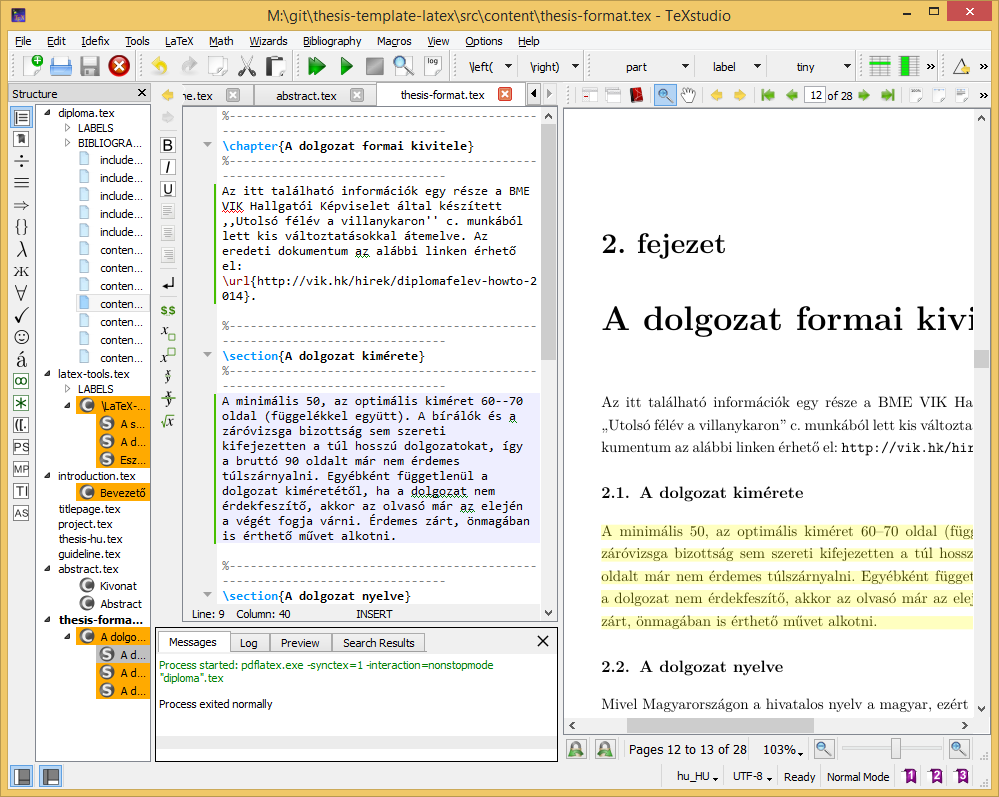
\includegraphics[width=150mm, keepaspectratio]{figures/TeXstudio.png}
\caption{A TeXstudio \LaTeX-szerkesztő.} 
\end{figure}

%----------------------------------------------------------------------------
\clearpage\section{Válasz az ,,Élet, a világmindenség, meg minden'' kérdésére}
%----------------------------------------------------------------------------
A Pitagorasz-tételből levezetve
\begin{align}
c^2=a^2+b^2=42.
\end{align}
A Faraday-indukciós törvényből levezetve
\begin{align}
\rot E=-\frac{dB}{dt}\hspace{1cm}\longrightarrow \hspace{1cm}
U_i=\oint\limits_\mathbf{L}{\mathbf{E}\mathbf{dl}}=-\frac{d}{dt}\int\limits_A{\mathbf{B}\mathbf{da}}=42.
\end{align}


%\label{page:last}
\end{document}
